\section{Aufbau der Wetterstation und deren Sensoren}
%\chapter{Aufbau der Wetterstation und Sensoren}


%% ############################################################################
%% Unterkapitel
%% ############################################################################
%\subsection{Übersicht über die verbaute Hardware}
Die Wetterstation Arbon verfügt über fünf Sensoren bzw. Sensor-Einheiten: Webcam, Kombi-Wetter-Transmitter, Wassertemperatur-Sensoren, Pegelsensor und Sonnenstrahlungssensor. Auf der Plattform im See befindet sich lediglich ein Schaltschrank mit Datenwandlern und keine Auswerteeinheit. Sämtliche Daten werden per TCP/IP über eine Glasfaserleitung an den Server geschickt. Abbildung \ref{img:schaltschrank} zeigt den schematischen Aufbau der Komponenten im Schaltschrank und die angeschlossenen Sensoren. Die Stromversorgung ist der Übersicht halber nicht dargestellt. Der Pegel- und Strahlungssensor wurden während dieser Arbeit ersetzt beziehungsweise hinzugefügt.

\begin{figure}[htbp]
	\centering
	\fbox{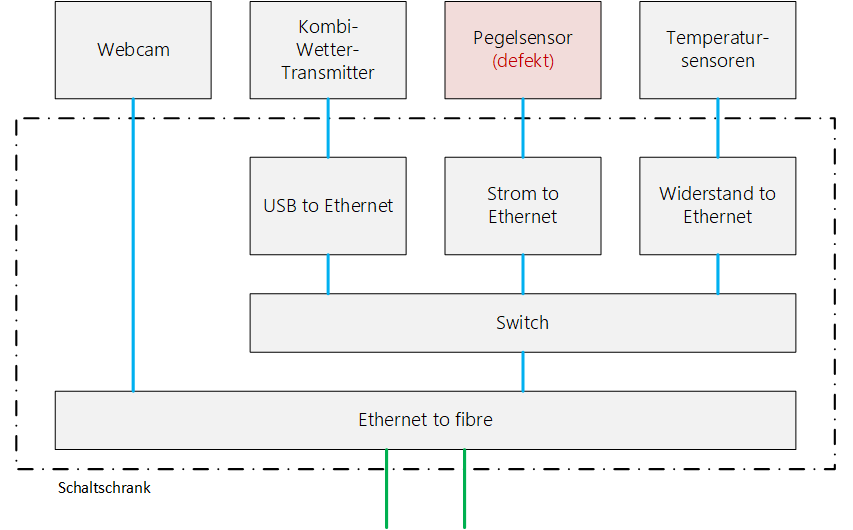
\includegraphics[width=\textwidth-2\fboxsep-2\fboxrule]{img/schaltschrank.png}}
	\caption{Hardware-Schema der Wetterstation}
	\label{img:schaltschrank}
\end{figure}

%% ############################################################################
%% Unterkapitel
%% ############################################################################
\subsection{Sonnenstrahlungssensor}
Die Sonnenscheindauer dient der näherungsweisen Bestimmung der Einstrahlung an einem bestimmten Ort und gibt gleichzeitig Hinweise auf Zeit und Stärke der Bewölkung. Sie diente ursprünglich der Charakterisierung von Kurorten. Dabei wurde die psychologische Wirkung von Sonnenlicht auf das menschliche Wohlbefinden hervorgehoben. Auch heute noch werden die Sonnenstunden verwendet um touristische Ziele zu fördern.

\noindent
Zur Messung der Sonnenstunden gibt es gemäss \flqq Guide to Meteorological Instruments and Methods of Observation (WMO)\frqq ~\cite{WMO2014Gtmi} fünf Messprinzipien, wobei die pyranometrische Methode die einfachste und kostengünstigste Methode darstellt. Gemäss WMO, Kapitel 8.1.4, kann die Sonnenscheindauer eines Orts durch die Messung der entsprechenden globalen Sonnenstrahlung\ $G$ abgeschätzt werden. Die Globalstrahlung wird dabei von einem Pyranometer gemessen.

\subsubsection{Funktionsprinzip eines Pyranometers}
Das Pyranometer basiert auf dem Messprinzip eines Thermoelements, wie in Abbildung \ref{img:pyranometer}  dargestellt. Die eintreffende Strahlung trifft auf einen Absorber, welcher erwärmt wird. Die Wärme fliesst dann über das Gehäuse an die Umgebung ab. Die Strahlungsleistung ist proportional zum Wärmestrom beziehungsweise zur Temperaturdifferenz vom Absorber zum Gehäuse. Die Temperaturdifferenz wird mit Thermoelementen gemessen. Um die Signalspannung zu erhöhen werden mehrere Thermoelemente in Reihe zu einer Thermosäule geschalten. Durch das thermische Messprinzip ist ein Pyranometer träge. Die Verzögerung liegt bei wenigen Sekunden. Das schwarz-poröse Absorbermaterial muss eine hohe Langzeitstabilität insbesondre gegenüber kurzwelliger Strahlung aufweisen.

\begin{figure}[htbp]
	\centering
	\fbox{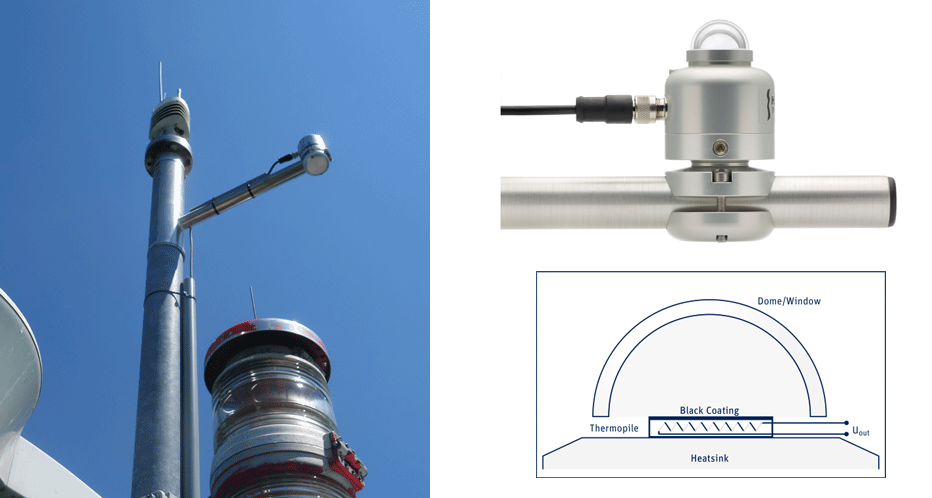
\includegraphics[width=\textwidth-2\fboxsep-2\fboxrule]{img/pyranometer.png}}
	\caption{Pyranometer}
	\label{img:pyranometer}
\end{figure}
%Quelle: http://www.kippzonen.com/News/572/The-Working-Principle-of-a-Thermopile-Pyranometer#.WzuK8C35ybg

\subsubsection{Berechnung der Sonnenscheindauer}
Die (relative) Sonnenscheindauer beschreibt den Anteil der tatsächlichen an der effektiv möglichen Sonnenscheindauer in Prozent. Durch sie kann man Sonnenscheinverhältnisse verschiedener Gebiete vergleichen. Gemäss ANNEX 8.B. der Richtlinie ~\cite{WMO2014Gtmi} kann die Sonnenscheindauer aus den minütlichen Messwerten der Globalstrahlung berechnet werden. Dazu muss zuerst der Schwellwert, wie in \ref{eq:Sonnenstunden} dargestellt, berechnet werden. Der Zähler für die Sonnenstunden wird um eine Minute erhöht, wenn der Messwert grösser ist als der Schwellwert und der Sonnenwinkel mindestens 3 Grad beträgt.\newline

\begin{equation}
\label{eq:Sonnenstunden}
G_{thr} = A + B * cos(\frac{360*d}{24*365}) * 1080 * sin(h)^{1.25}
\end{equation}

wobei:
\begin{conditions}
G_{thr}  &  Schwellwert der Globalstrahlung \\
d        &  Laufende Stunde seit Anfang Jahr \\
h        &  Elevationswinkel der Sonne in Grad \\
A        &  empirisch bestimmter Koeffizient (0.65) \\
B        &  empirisch bestimmter Koeffizient (0.15) \\
\end{conditions}

%Die physikalische Größe der Sonnenscheindauer (SD) ist Zeit. Die verwendeten Einheiten sind Sekunden oder Stunden.
%Der Messzeitraum (Tag, Dekade, Monat, Jahr usw.) ist ein wichtiger Zusatz zur Einheit.

\noindent
Wenn der Winkel $h$ grösser oder gleich 3 Grad ist, und der gemittelte Minutenwert der Solarstrahlung höher ist als der Schwellwert, wird der Zähler für die Sonnenstunde um eine Minute erhöht.

%Guten Tag Frau Bilgery,
%scheint grössere Abweichungen zu geben. Habe es mit zwei anderen Datensätzen versucht mit dem ähnlichen Ergebnis.
%
%Im beiliegenden File habe ich die Strahlung bei einer Sonnenhöhe <3 Grad auf Null gesetzt, d.h. Morgen und Abendstunden werden nicht berücksichtigt. Fehler mit Division von sin(h) gibt es dann auch nicht.
%Für Buchs ist dies zulässig da die umliegenden Berge über einem Höhenwinkel von 3 Grad liegen. Dies wird aber in der Literatur auch für südliche Regionen ohne Berge durchgeführt. D.h. dies ist eine Massnahme. Weitere Massnahme ist die Reduktion der Faktoren A und B bis die Werte übereinstimmen.
%
%Faktor B-Reduktion kann beurteilt werden, wenn ein Sommertag und Wintertag betrachtet wird, da dieser die Saisonalität bestimmt.

\begin{figure}[htbp]
	\centering
	\fbox{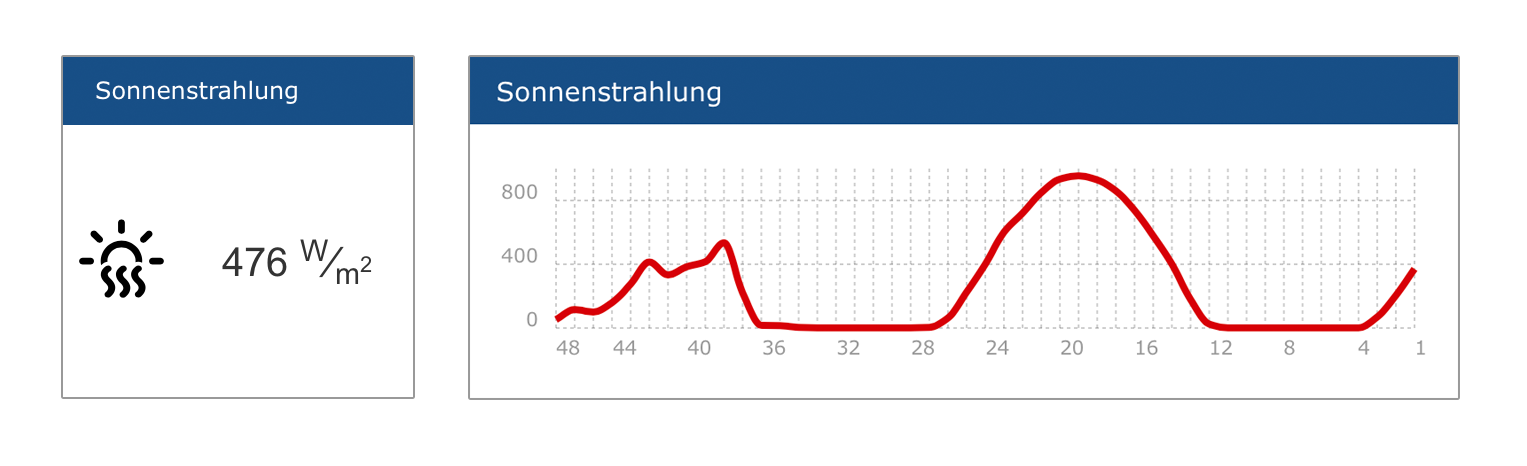
\includegraphics[width=\textwidth-2\fboxsep-2\fboxrule]{img/radiation}}
	%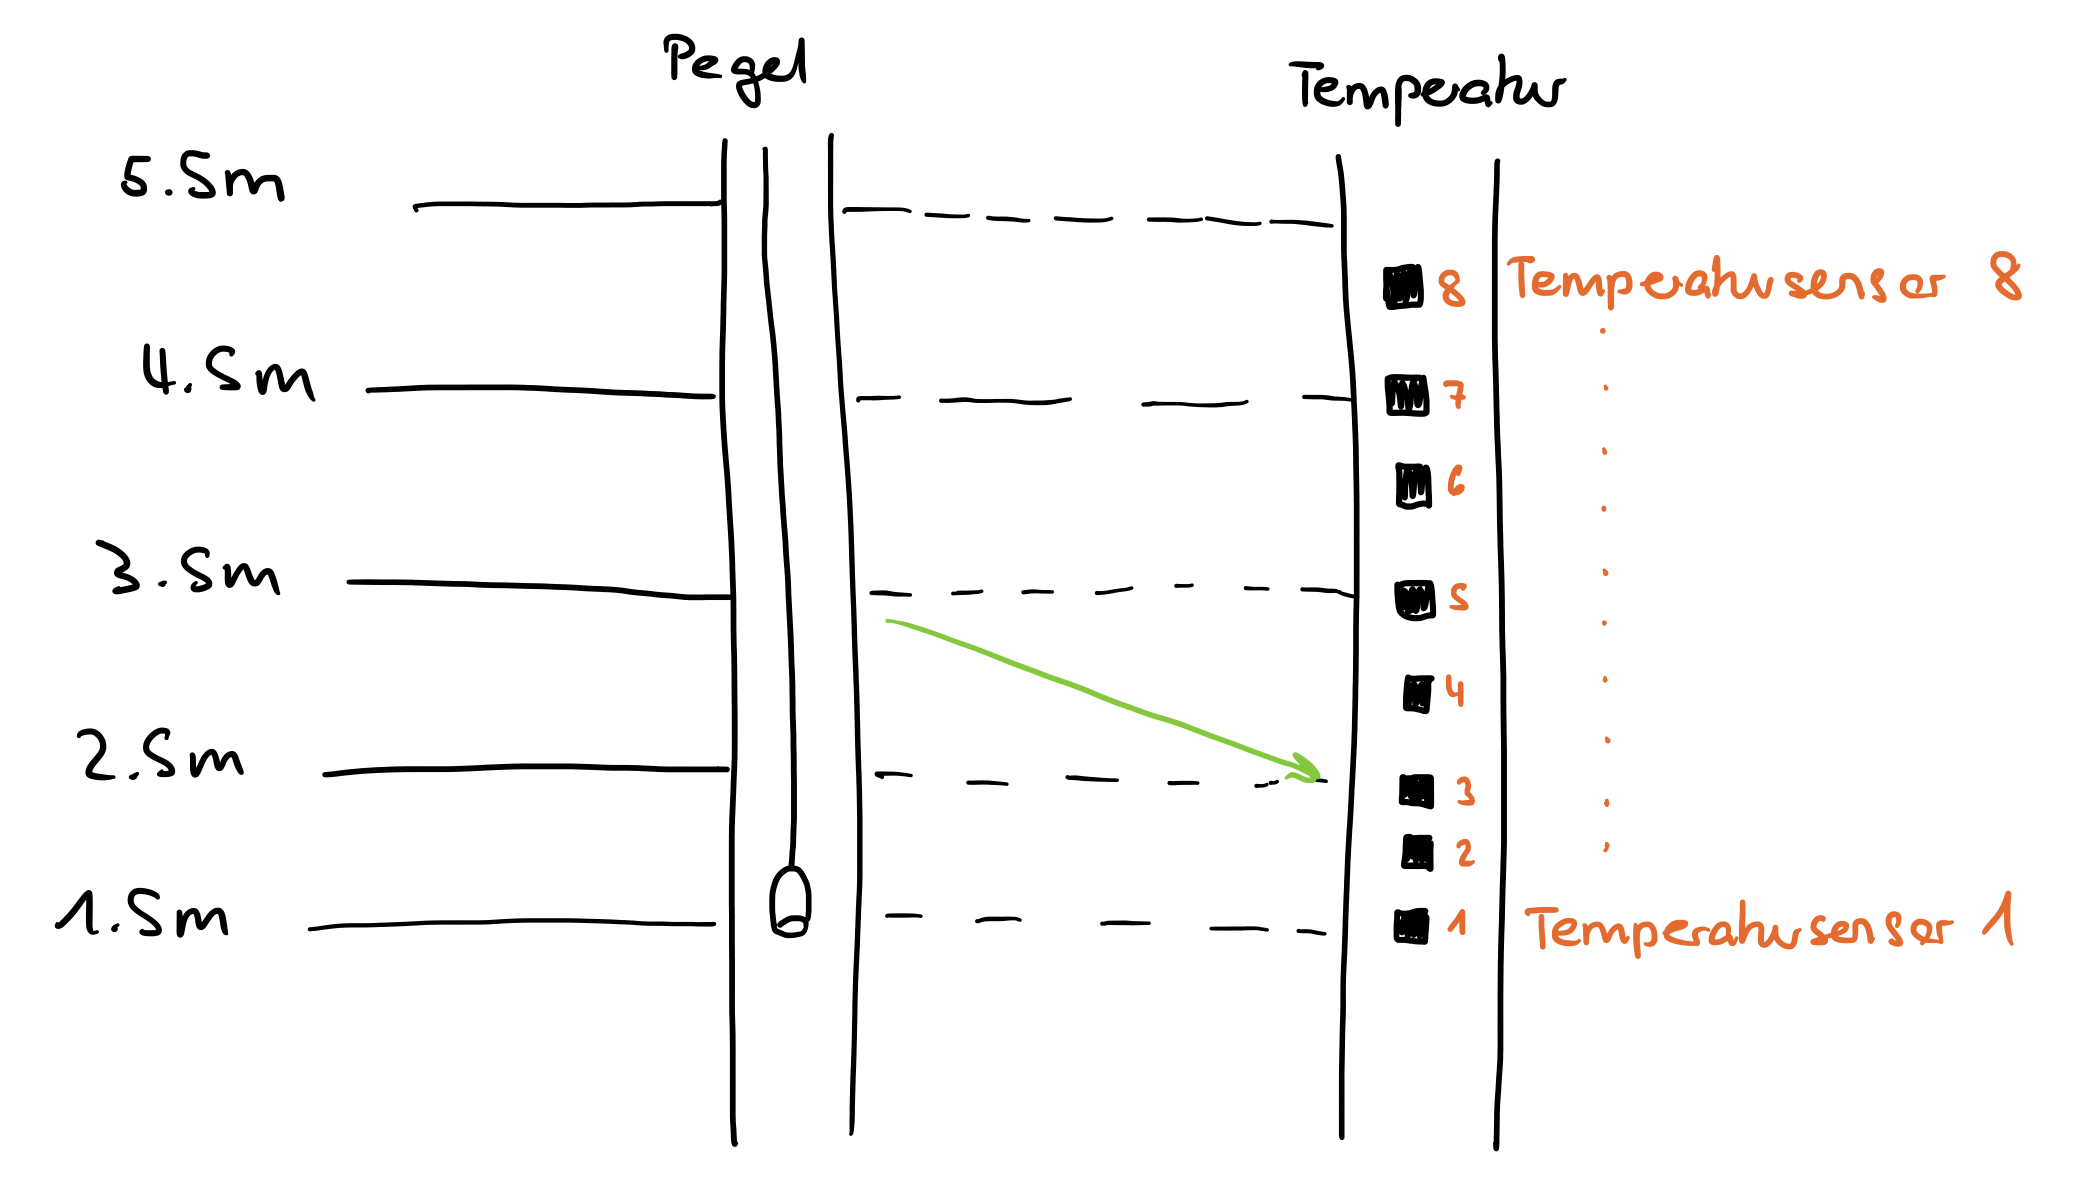
\includegraphics[width=0.9\linewidth]{img/wassertempsensoren.png}
	\caption{Darstellung des aktuellen Messwerts und des Strahlungsverlaufs}
	\label{img:radiation}
\end{figure}



\subsubsection{Verwendung für PV-Anlagen}
Das webbasierte Tool PVGIS\footnote{\url{http://re.jrc.ec.europa.eu/pvgis/apps4/pvest.php}}, welches durch das europäische Joint Research Centre (JRC) entwickelt wurde, ist \textit{das} Tool wenn es darum geht den Ertrag einer PV-Anlage vorherzusagen. Die Daten basierend auf Interpolationen von Messungen von Boden-Messstationen. Es liegt nahe diese Berechnung mit unseren Messwerten zu vergleichen. PVGIS berechnet für den Standort Arbon Werte gemäss Abbildung \ref{img:pvgis}.

\begin{figure}[htbp]
	\centering
	\fbox{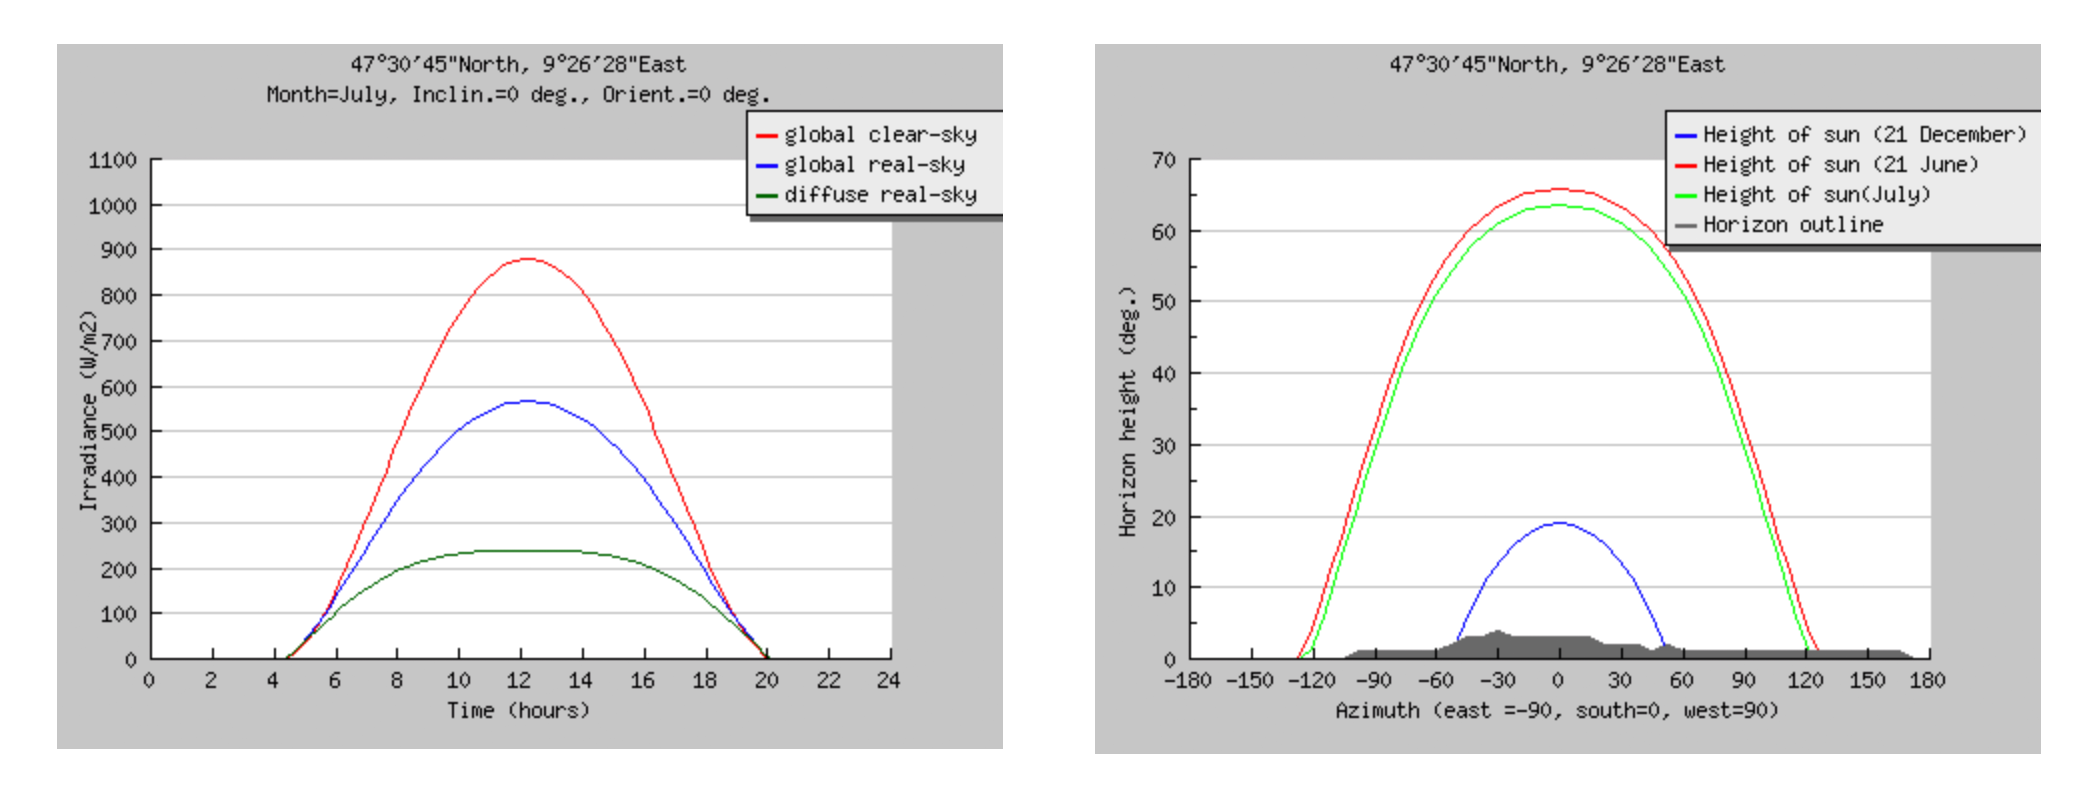
\includegraphics[width=\textwidth-2\fboxsep-2\fboxrule]{img/pvgis}}
	\caption{Pyranometer}
	\label{img:pvgis}
\end{figure}




%% ############################################################################
%% Unterkapitel
%% ############################################################################
\subsection{Pegelsensor und Wellenhöhenmessung}
Die ursprüngliche Wetterstation verwendete einen hydrostatischen Drucksensor für die Messung des Wasserstands (Pegel). Der Drucksensor lieferte aber nach zehn Jahren Betrieb keine plausiblen Werte mehr, weshalb er ersetzt werden musste.

\subsubsection{Auswahl eines geeigneten Pegelsensors}
Für die Messung des Bodensee-Pegels wurden verschiedene Messprinzipien verglichen, mit dem Hintergedanken die Pegelmesswerte ebenfalls zur Messung der Wellenhöhe verwenden zu können. Die Zusammenfassung der Resultate ist in der Tabelle \ref{tbl:pegelsensoren} aufgelistet.

\begin{table}[htbp!]
\label{tbl:pegelsensoren}
\caption{Gegenüberstellung der verschiedenen Pegelmess-Prinzipien}
\setlength\extrarowheight{3pt} % for a more "open" look
\begin{tabularx}{\textwidth}{|>{\RaggedRight\hspace{0pt}}p{1.5cm}||X|X|}
\hline
 & \bfseries\large Vorteile & \bfseries\large Nachteile\\

\hline
\textbf{Hydrostatisch}
&
\begin{itemize}[nosep,leftmargin=*]
\item einfache Auswertung
\item mechanische Dämpfung
\item sehr kleiner Energieverbrauch
\end{itemize}
&
\begin{itemize}[nosep,leftmargin=*]
\item anfällig auf Verschmutzung
\item keine Wellenmessung möglich
\end{itemize}\\

\hline
\textbf{Ultraschall}
&
\begin{itemize}[nosep,leftmargin=*]
\item berührungslos
\item geringer Energiebedarf
\end{itemize}
&
\begin{itemize}[nosep,leftmargin=*]
\item anfällig auf Wind
\end{itemize}\\

\hline
\textbf{Radar}
&
\begin{itemize}[nosep,leftmargin=*]
\item windunabhängig
\item berührungslos
\end{itemize}
&
\begin{itemize}[nosep,leftmargin=*]
\item zu geringe Auflösung für Wellenhöhe
\item hoher Energiebedarf
\end{itemize}\\

\hline
\textbf{TOF}
&
\begin{itemize}[nosep,leftmargin=*]
\item Wellenhöhe messbar
\item berührungslos
\end{itemize}
&
\begin{itemize}[nosep,leftmargin=*]
\item komplexe Auswertung
\end{itemize}\\

\hline
\textbf{Boje}
&
\begin{itemize}[nosep,leftmargin=*]
\item Wellenhöhe messbar
\end{itemize}
&
\begin{itemize}[nosep,leftmargin=*]
\item wartungsintensiv
\item Batteriebetrieb
\end{itemize}\\

\hline
\end{tabularx}
\end{table}

\noindent
Die Einfachheit und Robustheit des hydrostatischen Sensors überwog, sodass der alte Drucksensor durch das gleiche Produkt ersetzt wurde.

\subsubsection{Definition des Pegel Konstanz}
Die Uferlinie des Bodensees wurde 1990 von der IGKB bei Mittelwasserstand festgelegt. Der Pegelstand in Konstanz ist ein Relativmaß. Es bezieht sich auf den Pegelnullpunkt, der in Konstanz bei 391,89m ü NN liegt. Der Pegel Romanshorn gibt die geodätische Höhe des Wasserstandes wieder\footnote{\url{http://www.bodensee-hochwasser.info/IGKB/umrechnung.html}}. Der Zusammenhang der verschieden Pegelgrössen ist in Abbildung \ref{img:pegelKonstanz} dargestellt. Links oben befindet sich die Skala für den Pegel Konstanz.

\begin{figure}[htbp]
	\centering
	\fbox{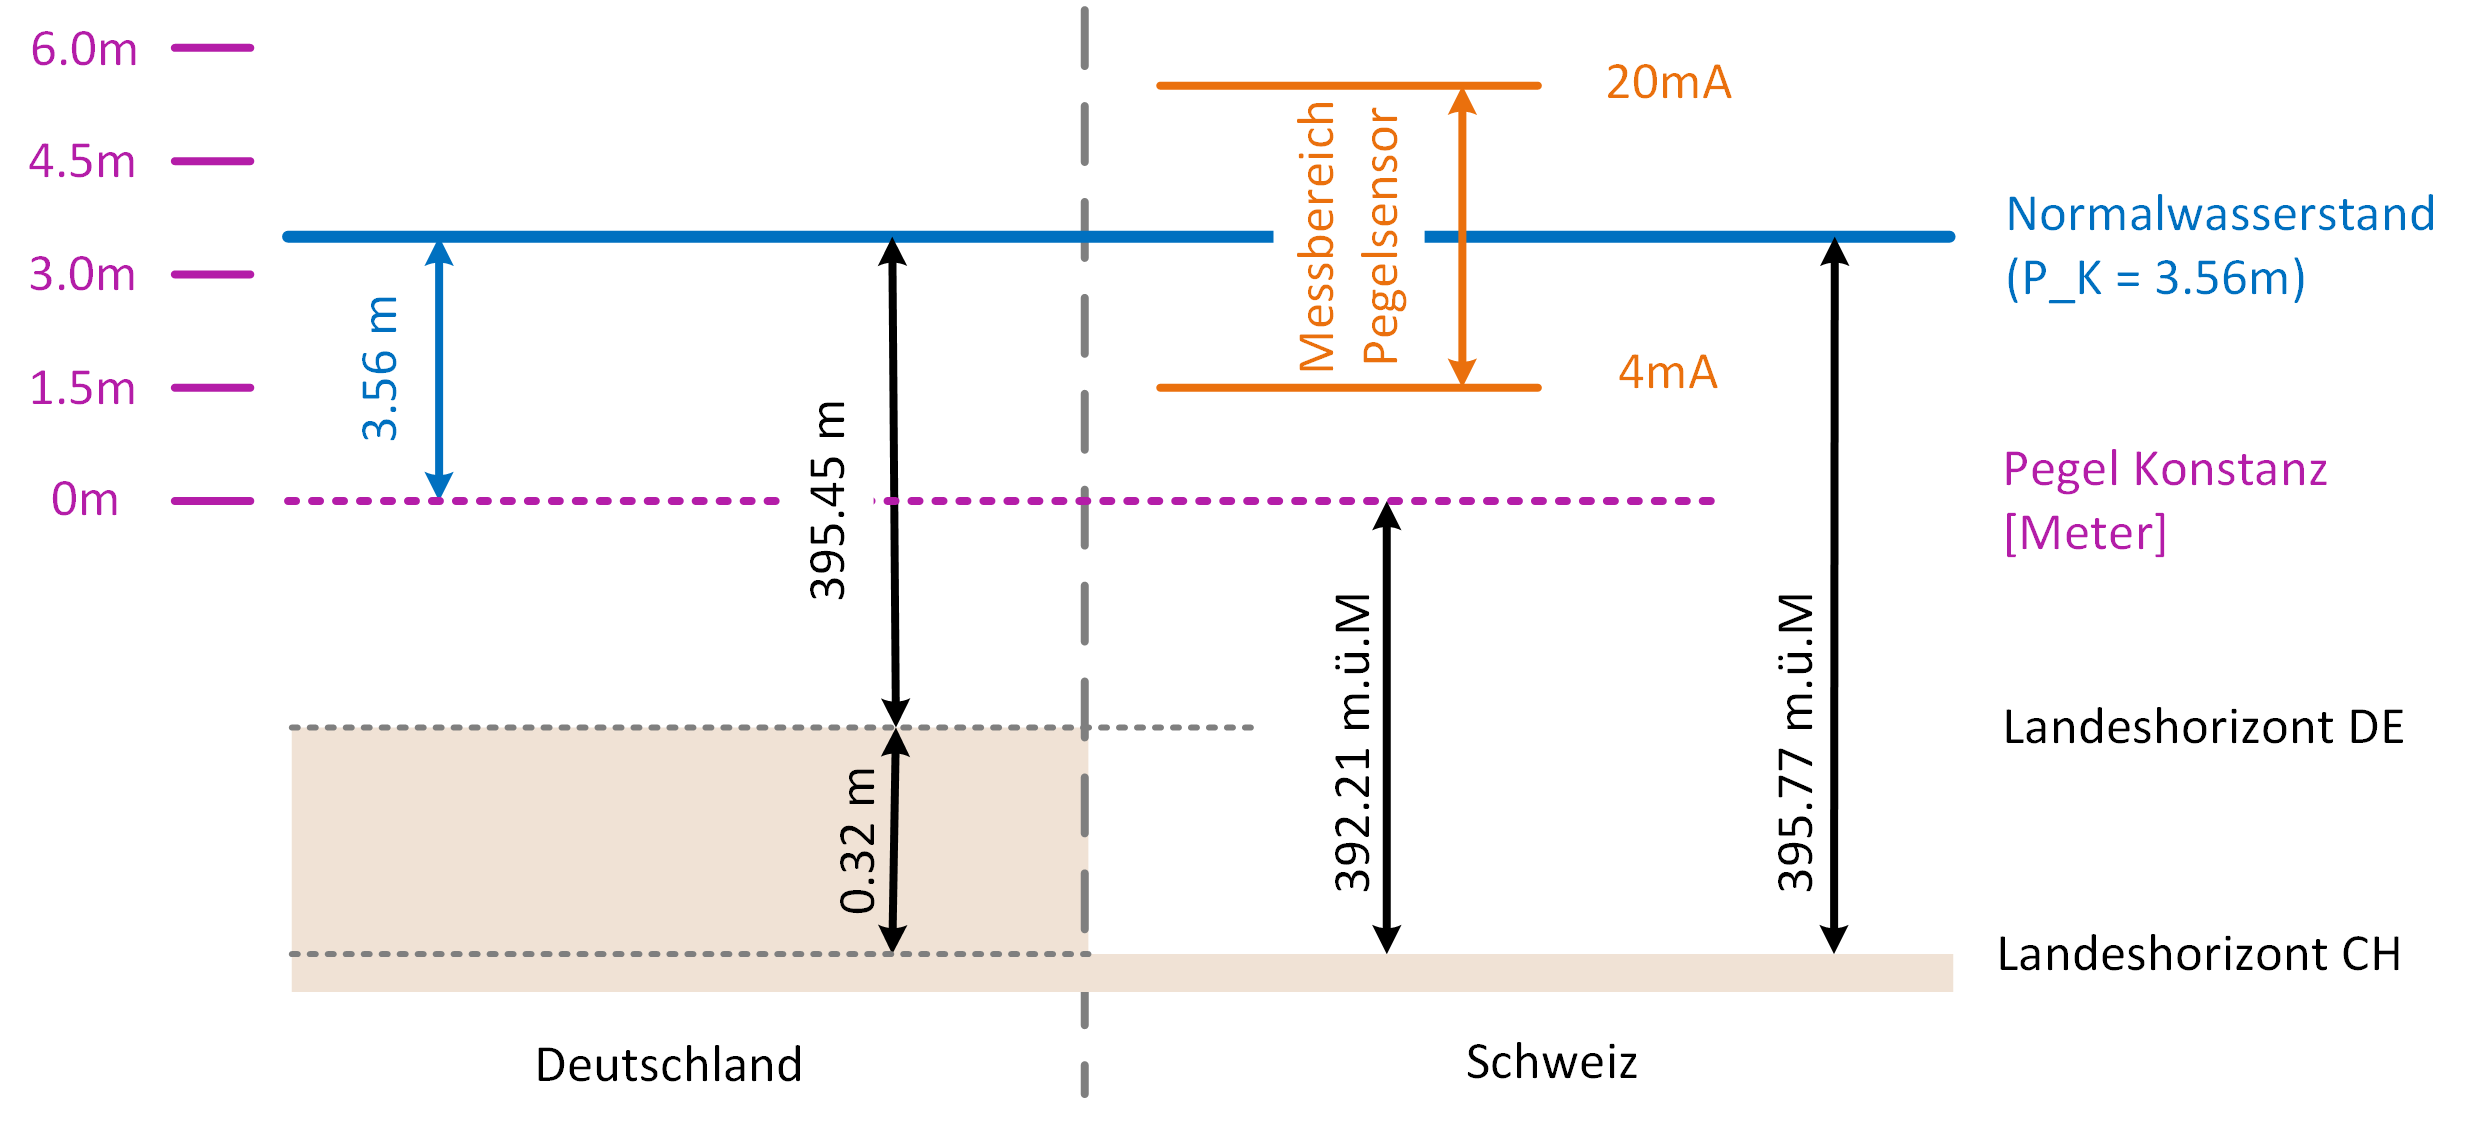
\includegraphics[width=\textwidth-2\fboxsep-2\fboxrule]{img/pegelKonstanz}}
	%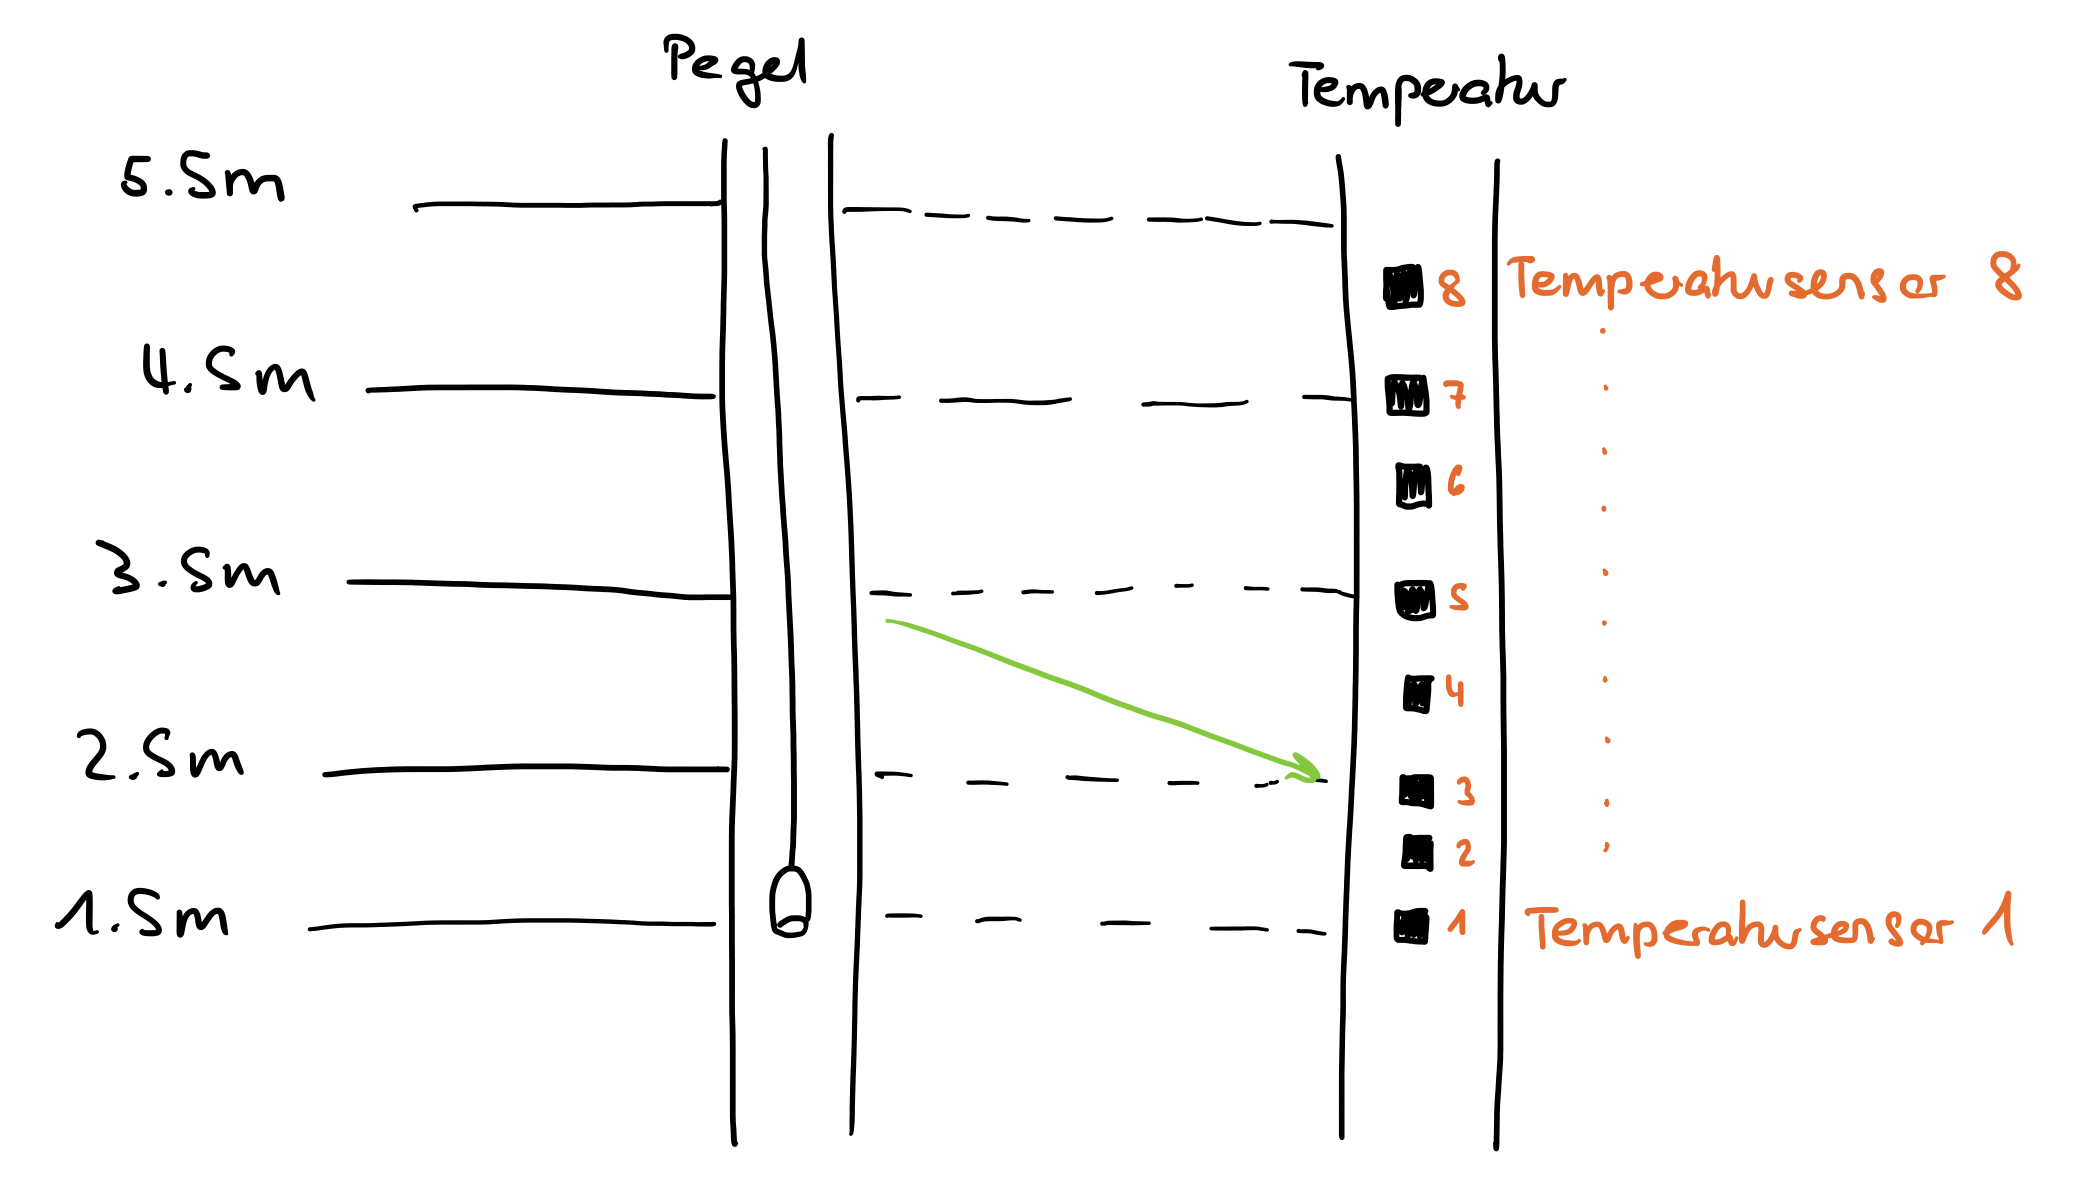
\includegraphics[width=0.9\linewidth]{img/wassertempsensoren.png}
	\caption{Berechnung des Pegel Konstanz und Messbereich des Sensors}
	\label{img:pegelKonstanz}
\end{figure}

Der Pegelsensor liefert 4...20mA bei einer Messhöhe von 4 Meter. Der Pegelsensor ist 1.75 Meter über dem Pegelnullstand angebracht.
Die Berechnung des Pegel Konstanz aus dem Messwert erfolgt gemäss der Formel \ref{eq:Pegelformel}.

\begin{equation}
\label{eq:Pegelformel}
P_{K} = m*x + q = 4/16 * x + 0.75
\end{equation}

\begin{equation}
\label{eq:Pegelmin}
P_{g,u}= P_{K}(x=4)= 4*0.25 + 0.75 = 1.75
\end{equation}

\begin{equation}
\label{eq:Pegelmax}
P_{g,o} = P_{K}(x=20)= 20*0.25 + 0.75 = 5.75
\end{equation}

wobei:
\begin{conditions}
P_{K}    &  Pegel Konstanz [m]\\
P_{g,u}   &  Tiefster messbarer Pegel [m]\\
P_{g,o}   &  Höchster messbarer Pegel [m]\\
x        &  Messwert [mA]\\
m        &  Auflösung des Sensors [m/mA] (0...4m bei 4...20mA)\\
q        &  Offset [m] \\
\end{conditions}

Die Messdaten des Pegelsensors können per Web-Schnittstelle abgefragt werden, wie in Listing \ref{lst:curlPegel} aufgezeigt. Da die Geräte, die diesen Dienst zur Verfügung stellen nur schwach gegen unerwünschte Zugriffe geschützt sind, wurde die Firewall der Wetterstation so konfiguriert, dass nur vom Hostpoint-Server aus die Abfrage durchgeführt werden kann (IP-Regel).

\begin{lstlisting}[label=lst:curlPegel,caption=Abfrage des Pegelsensor-Wertes über das Hostpoint-Termianl, language=Python, style=htmlcssjs]
[igwetter@s34:~] $ curl http://webcam.wetter-arbon.ch:50506/single1
11,748 mA
\end{lstlisting}


\subsubsection{Definition der signifikaten Wellenhöhe}
Als Seegang bezeichnet man die winderzeugten Oberflächenwellen des Meeres. Da sich der Seegang in der Natur als eine Überlagerung vieler Einzelwellen darstellt, werden zu dessen Beschreibung statistische Größen wie z.B. die signifikante Wellenhöhe verwendet. Die Definition einer signifikaten Wellenhöhe geht auf die visuelle Bestimmung einer charakteristischen, den Seegang beschriebenden Wellenhöhe zurück. Die signifikatnte Wellenhöhe wird gemäss der \textit{List of sea state parameters}\cite{1986Iahr} definiert als die mittlere Wellenhöhe der 33\% höchsten Wellen in einem repräsentativen Zeitraum (z.B. 20 Minuten).


%% ############################################################################
%% Unterkapitel
%% ############################################################################
\subsection{Wassertemperatur-Sensoren}
Die Wetterstation verfügt über acht Wasser-Temperatursensoren (PT100-Elemente), die im Abstand von 0.5m in einem Rohr angebracht sind. Die Wassertemperatur wird standardmässig einen Meter unter der Wasseroberfläche gemessen.
% \Diskussionspunkt{- Wo ist Wassertemperatur definiert? }\newline

\subsubsection{Auswahl des richtigen Temperatursensors anhand des Pegels}
Damit der richtige Temperatursensor ausgewählt werden kann, muss der Pegel bekannt sein. Abbildung \ref{img:wassertempsensoren} zeigt das Prinzip schematisch auf. Mittels Cronjob werden sämtliche Temperatursensoren ausgelesen und in einem Array gespeichert. Anschliessend wird mit Hilfe des Pegelwerts der korrekte Wert entnommen, wie in Listing \ref{lst:tempSelect} beispielhaft aufgezeigt.

\begin{lstlisting}[label=lst:tempSelect,caption=Auswahl des richtigen Temperatursensors, language=Python, style=py]
if waterlevel >= 3.5 and waterlevel <=4.0:
    watertemperature100cm  = float(temperatureArray[3])
    watertemperature50cm = float(temperatureArray[4])
\end{lstlisting}

\noindent
Die offizielle Wassertemperatur wird einen Meter unter der Wasseroberfläche gemessen. Für Schwimmer ist aber die Temperatur eine halben Meter unter der Wasseroberfläche interessanter, weshalb dieser Wert ebenfalls ausgelesen und gespeichert wird. Das Schwimmbad Arbon bezieht bereits heute für ihre Webseite\footnote{\url{https://www.schwimmbad-arbon.ch}} die Wassertemperatur von der Wetterstation.


\begin{figure}[htbp]
	\centering
	\fbox{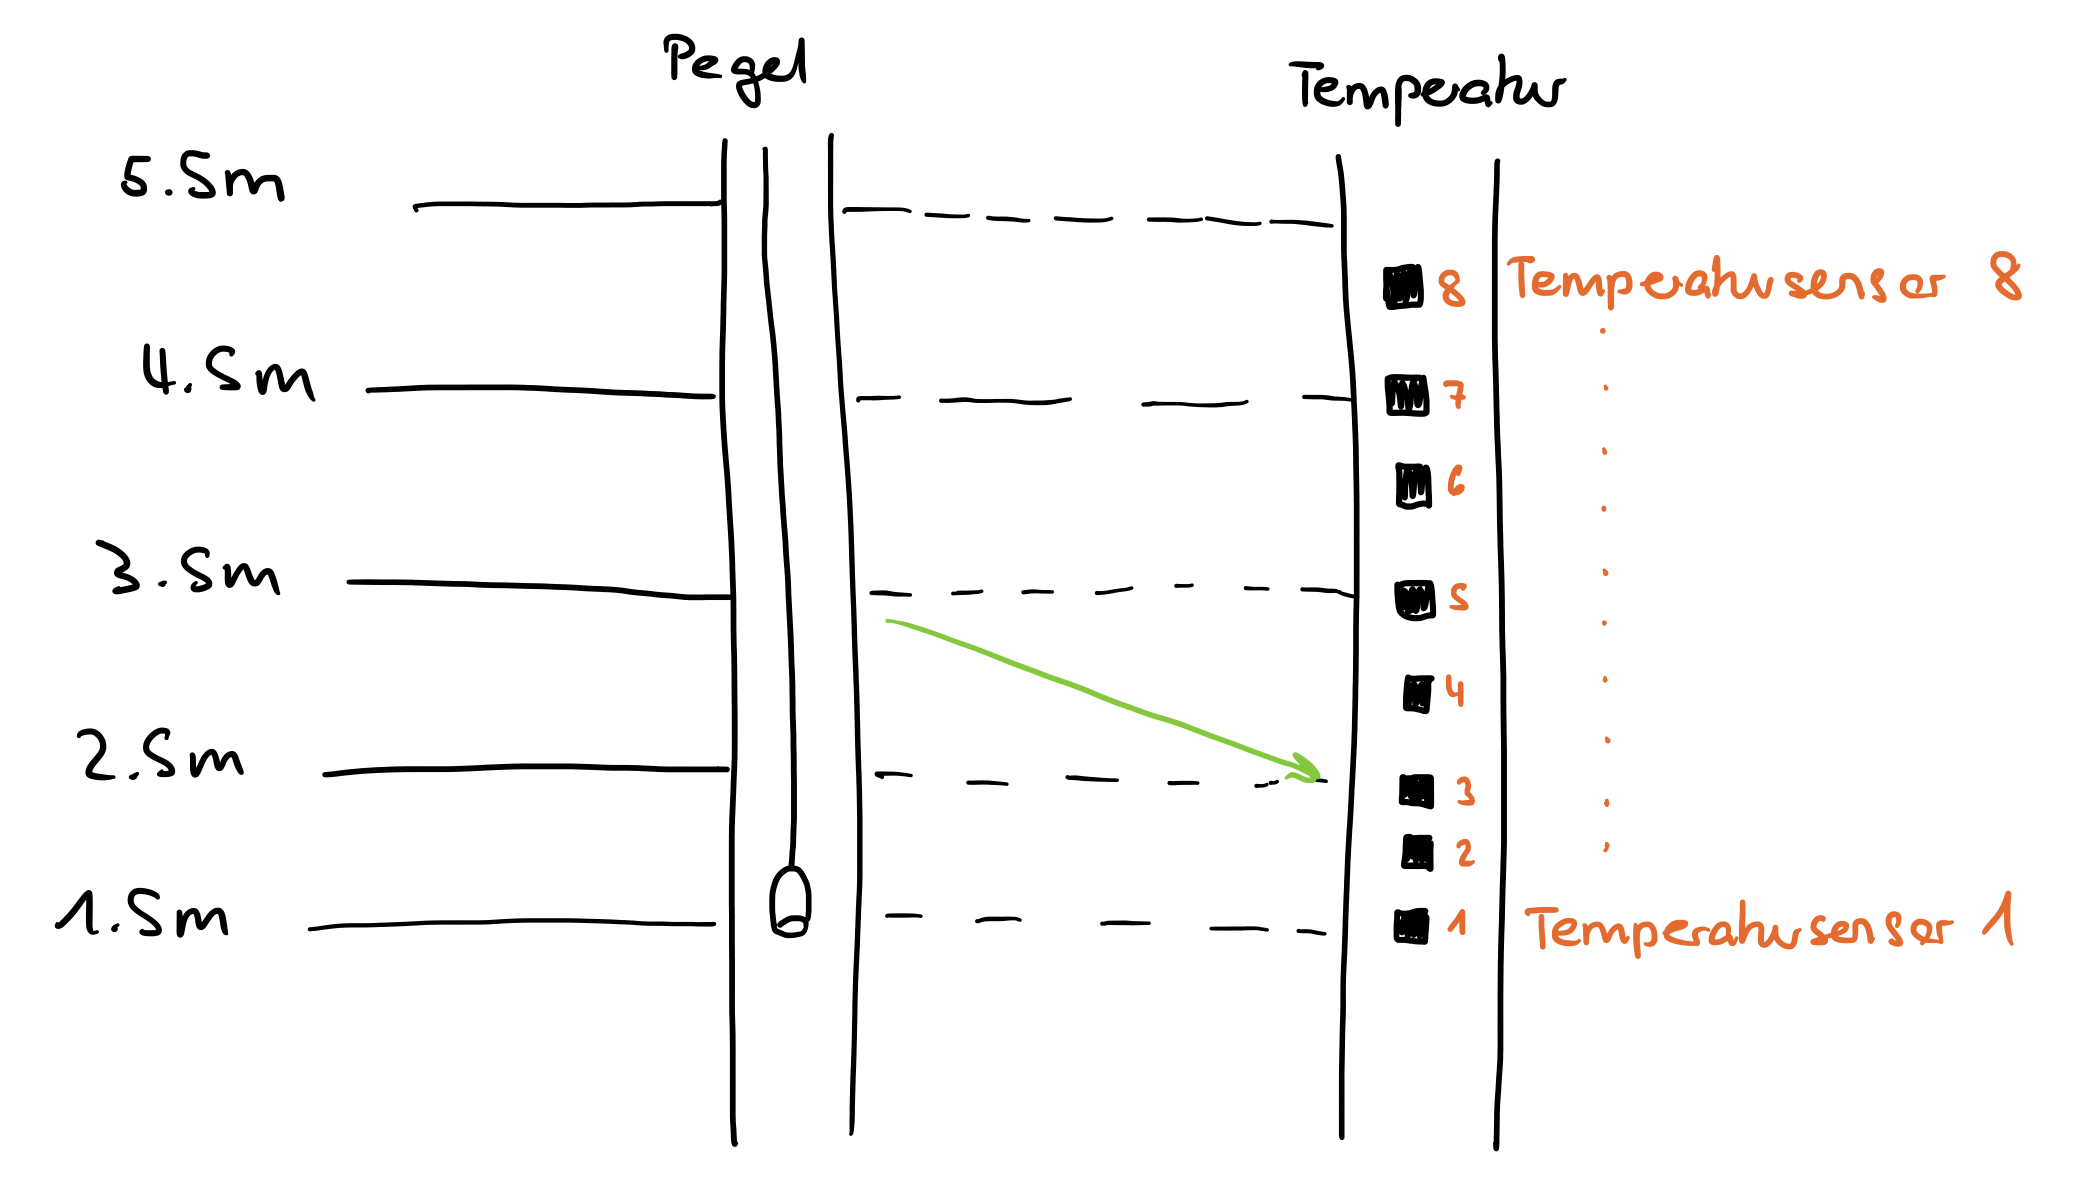
\includegraphics[width=\textwidth-2\fboxsep-2\fboxrule]{img/wassertempsensoren}}
	\caption{Zusammenhang zwischen Pegel und PT100-Temperaturwiderständen}
	\label{img:wassertempsensoren}
\end{figure}


\subsubsection{Annäherung des defekten PT100-Widerstands}
Die Temperatursensoren waren mehrere Jahre nicht in Betrieb. Es wurde deshalb während mehrerer Tag alle Temperaturdaten aufgezeichnet. Aus Auszug der Messdaten sind in Abbildung \ref{img:tempSensoren} dargestellt. Es lässt sich gut erkennen, dass die Sensoren 1 bis 4 sich im Wasser und die Sensoren 6 bis 8 über dem Wasser befinden. Beim Sensor 5 ist nicht klar ober er im oder über dem Wasser ist. Auf Grund der Messdaten lässt sich auch kein konstanter Offset gegenüber den benachbarten Sensoren erkennen.

\begin{figure}[htbp]
	\centering
	\fbox{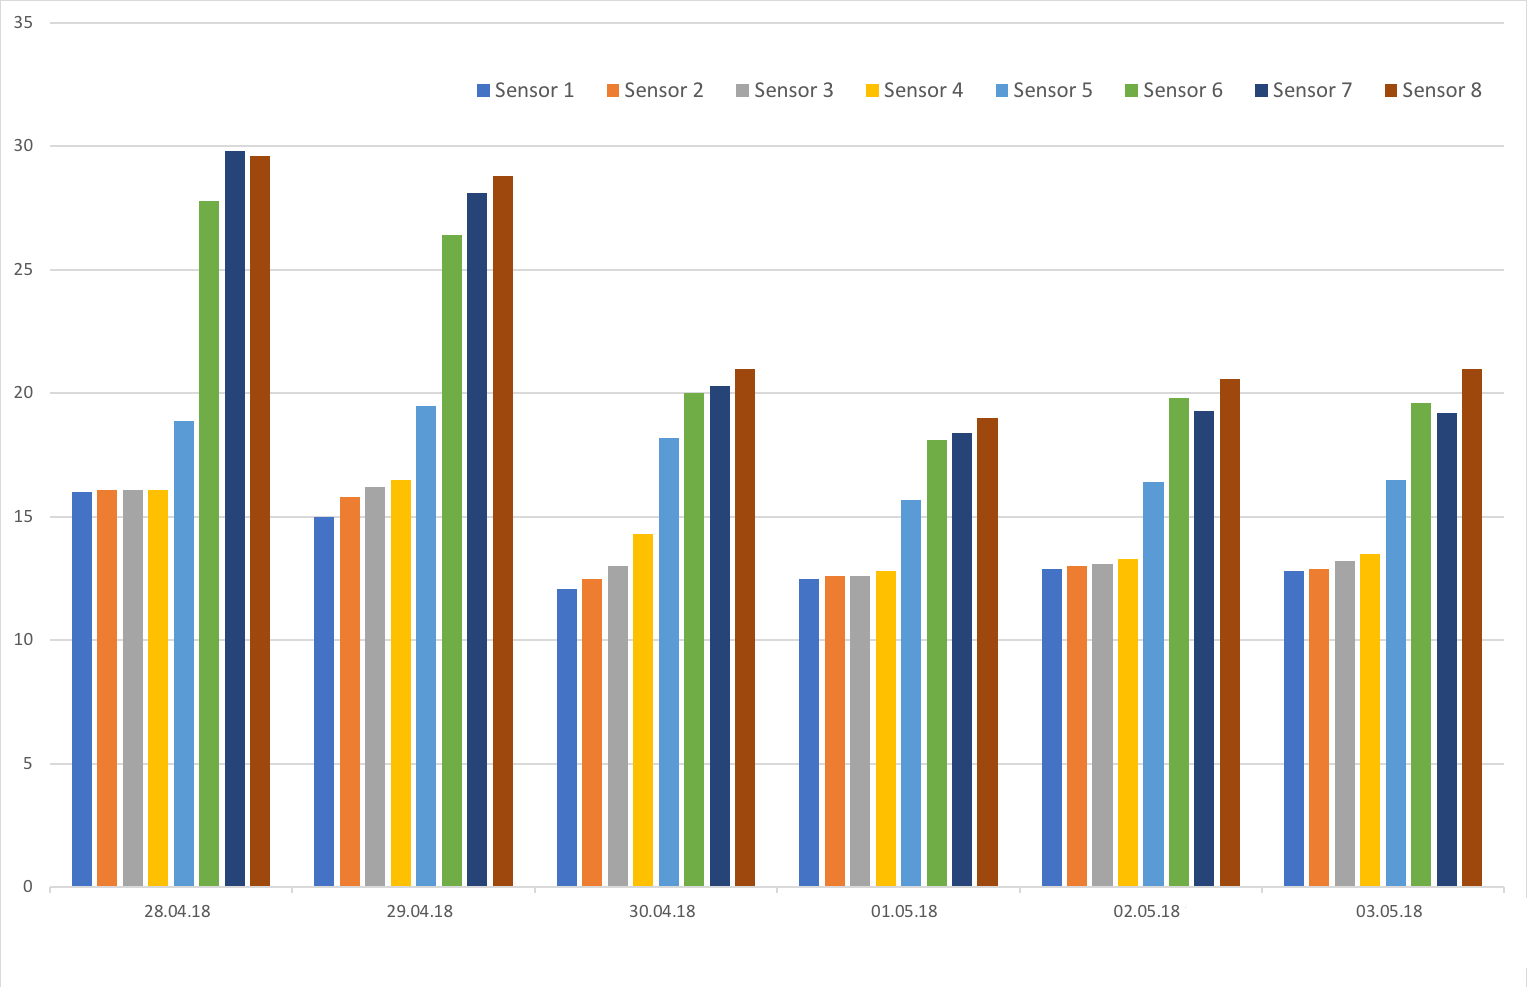
\includegraphics[width=\textwidth-2\fboxsep-2\fboxrule]{img/tempSensoren}}
	\caption{Messreihe aller Temperatursensoren}
	\label{img:tempSensoren}
\end{figure}

Der fehlende bzw. falsche Wert wurde trotzdem durch einen Offset angenähert.Ein Offset von drei Grad hat sich als meistens korrekt erwiesen. Der Offset wird direkt beim Auslesen der Temperaturdaten abgezogen, wie in Listing \ref{lst:tempOffset} aufgezeigt.

\begin{lstlisting}[label=lst:tempOffset,caption=Offset des defekten Temperatusensors, language=Python, style=py]
temperatureArray[4] = float(temperatureArray[4])-3.0
\end{lstlisting}
